\documentclass[11pt,twocolumn]{article}
\usepackage[margin=0.72in]{geometry}
\usepackage{amsmath,amssymb,amsthm}
\usepackage{booktabs}
\usepackage{graphicx}
\usepackage{hyperref}
\usepackage{xcolor}
\usepackage{enumitem}

\hypersetup{
  colorlinks=true,
  linkcolor=blue!60!black,
  citecolor=green!45!black,
  urlcolor=blue!65!black
}

\newtheorem{proposition}{Proposition}
\newtheorem{definition}{Definition}

\newcommand{\ZZ}{\mathbb{Z}}
\newcommand{\QQ}{\mathbb{Q}}
\newcommand{\NN}{\mathbb{N}}

\title{\textbf{Machine-Checked Exact-Rational Tower Transition, $d$-Closed Barrier, and Outward-Witness Certificates for Majority Bootstrap Percolation}}
\author{Lluis Eriksson\thanks{Independent researcher; manuscript prepared with transparent AI assistance via Google Antigravity. Source code, Lean~4 proofs, and exact certificates: \url{https://github.com/lluiseriksson/bootstrap-tower-transition-certificates}.}}
\date{November 25, 2026}

\begin{document}
\maketitle

\begin{abstract}
Vyacheslav Koval and Yuval Peres (\texttt{arXiv:2611.33087}, November 24, 2026) resolved the high-dimensional phase transition of majority ($d$-neighbour) bootstrap percolation on the discrete torus $\ZZ_n^d$, proving a sharp \emph{tower transition} (Theorem~1.1): when $H(n)/d \to \rho \in [0,1]$ (with $H(n)=\log_2^\ast n$), the critical density converges to $p_\rho = (1-\rho)/(2-\rho)$, recovering Morris's $p=1/4 \leftrightarrow \rho=2/3$ threshold (Corollary~1.2) and contrasting sharply with the dyadic box limit $p_c([n]^d) \to 1-2^{-m}$ at $n/d = 1/m$ (Eq.~1.2). We present a machine-checked, zero-floating-point formalization and exact-$\QQ$ certificate auditor for the algebraic, combinatorial, barrier-closure, and finite-scale geometric core of these results. First, an 18-theorem zero-dependency Lean~4 kernel (\texttt{BootstrapTowerTransition.lean}, Lean~4.35.0; 0~\texttt{sorry}, 0~warnings, 0~\texttt{Classical.choice}, 3 zero-axiom theorems) formalizes the tetration tower $T_0,\dots,T_4$, strict monotonicity, the exact cleared bijection $p_\rho \leftrightarrow \rho_p$, Morris's $(2/3,1/4)$ point, expected-support balance $v+(2d-v)p=d$, inductive Eq.~(2.3) $d$-closed layer closure over arbitrary lists, abstract monotone closure, Lemma~2.1 geodesic overlap margins, Eq.~(1.2) dyadic box gaps $1-2^{-m} > 1/2$, and Lemma~2.3 rectangle-merge hull bounds. Second, \texttt{BOOTSTRAP-TOWER-CERT-1.0} audits four exact-$\QQ$ modes—tower-curve bijections, exact finite $\ZZ_n^d$/$[n]^d$ filling and Eq.~(2.3) $d$-closed barriers, exact rational Lemma~2.1 binomial tails $w_0$, and dyadic box limits with $\ell_\infty > 2t$ separated rectangles—replaying 16 canonical certificates in $0.036$--$0.446\,\mathrm{ms}$ and rejecting 60/60 live adversarial forgeries.
\end{abstract}

\section{Introduction}
In majority ($r=d$) bootstrap percolation~\cite{chalupa1979bootstrap,balogh2009majority,balogh2012sharp,morris2017bootstrap}, vertices of a finite lattice graph $\ZZ_n^d$ or $[n]^d$ are initially infected independently with probability~$p$, and at each discrete round any healthy vertex with at least~$d$ infected nearest neighbours becomes permanently infected. Koval and Peres~\cite{koval2026tower} uncovered a striking \emph{tower transition} on the $d$-dimensional torus $\ZZ_n^d$: whenever $H(n)/d \to \rho \in [0,1]$—where $H(n)=\log_2^\ast n = \min\{k : n \le T_k\}$ is the iterated base-2 logarithm inverting the tetration tower $T_0=1, T_{k+1}=2^{T_k}$—the critical filling probability converges to
\begin{equation}
  p_\rho = \frac{1-\rho}{2-\rho} \quad \Longleftrightarrow \quad \rho_p = \frac{1-2p}{1-p},
  \label{eq:tower}
\end{equation}
resolving Morris's $p=1/4$ benchmark at $\rho = 2/3$ (Corollary~1.2). By contrast, on the open box $[n]^d$ with $n/d = 1/m$, boundary corners of degree~$d$ force a strictly super-half dyadic threshold $p_c([n]^d) \to 1 - 2^{-m}$ (Eq.~1.2 of~\cite{koval2026tower}).

The subcritical lower-bound architecture of~\cite{koval2026tower} rests on deterministic and exact rational pillars: expected-support balance $v + (2d-v)p = d$, the multi-layer $d$-closed barrier $B(V) = I \cup E_0 \cup \dots \cup E_{h-1}$ (Eq.~2.3) guaranteeing $A_\infty \subseteq B(V)$ whenever $E_h(V) \subseteq B(V)$, the exact binomial outward-witness probability $w_0$ (Lemma~2.1, Eq.~2.4), and $\ell_\infty > 2t$ separated-rectangle merges (Lemma~2.3). Auditing these finite mechanisms over exact $\ZZ/\QQ$ arithmetic eliminates floating-point rounding in deep binomial tails ($>140$-bit numerators) and produces independently replayable proofs of both finite filling and barrier containment.

\paragraph{Contributions and Scope.}
We formally verify and audit the finite algebraic, combinatorial, barrier-closure, and rational-tail core of~\cite{koval2026tower}. We explicitly scope our Lean~4 formalization away from the asymptotic probabilistic couplings, multiscale renormalization, and infinite-dimension limit theorems of~\cite{koval2026tower}:
\begin{enumerate}[leftmargin=*,nosep]
  \item \textbf{Zero-dependency Lean~4 kernel (\S\ref{sec:lean}):} 18 constructive theorems in \texttt{BootstrapTowerTransition.lean} (Lean~4.35.0~\cite{demoura2021lean4}), 0~\texttt{sorry}, 0~warnings, 0~\texttt{Classical.choice}, 3 zero-axiom theorems.
  \item \textbf{Exact-$\QQ$ four-mode verifier (\S\ref{sec:certifier}):} \texttt{BOOTSTRAP-TOWER-CERT-1.0}, auditing tower bijections, exact finite bootstrap dynamics and Eq.~(2.3) $d$-closed barriers, exact rational Lemma~2.1 $w_0$ tails, and Eq.~(1.2)/Lemma~2.3 dyadic box and separated-rectangle certificates with zero floats.
  \item \textbf{Empirical atlas, exact filling polynomials, \& red-team audit (\S\ref{sec:results}):} 16 canonical certificates ($0.036$--$0.446\,\mathrm{ms}$), exhaustive $2^9$-configuration filling polynomials on $\ZZ_3^2$ vs.\ $[3]^2$, Eq.~(2.3) barrier census on $\ZZ_4^3$, exact-$\QQ$ $w_0$ decay sweeps ($d=10..32$), and 60/60 rejected live adversarial forgeries.
\end{enumerate}

\section{Tower Curve, $d$-Closed Barriers, and Outward Witnesses}\label{sec:prelim}
At infection density $p \in (0, 1/2)$, a vertex with $v$ forced neighbours and $2d-v$ independent Bernoulli($p$) neighbours has expected infected degree $v + (2d-v)p$, which equals the threshold~$d$ precisely at $v = \rho_p d$ where $\rho_p = (1-2p)/(1-p)$. On a finite graph $G=(\ZZ_n^d\text{ or }[n]^d)$ with initial seed set~$I$ and integers $h, g \ge 1$ satisfying $G_{\mathrm{bud}} := hg < d$, define the Eq.~(2.3) layers inductively:
\begin{equation}
\begin{aligned}
  E_0 &= \{v \notin I : \deg_I(v) \ge d - hg\}, \\
  E_i &= \{v : \deg_{E_{i-1}}(v) > g\} \quad (1 \le i \le h),
\end{aligned}
  \label{eq:barrier}
\end{equation}
and set $B(V) = I \cup E_0 \cup \dots \cup E_{h-1}$. Whenever $E_h \subseteq B(V)$, any vertex $v \notin B(V)$ has at most $d-hg-1$ neighbours in~$I$ and at most $g$ neighbours in each of $E_0,\dots,E_{h-1}$, hence $\deg_{B(V)}(v) \le d-1 < d$; thus $B(V)$ is $d$-closed and traps the entire percolation closure $A_\infty \subseteq B(V)$. In Lemma~2.1 (Eq.~2.4), for $g > 2h$ ($u = g-2h \ge 1$) and $H$ forced directions, the exact single-site outward-witness probability is
\begin{equation}
  w_0 = (1-p)\,\Pr\!\bigl[\mathrm{Bin}(2d-H,\, p) \ge d - hg - 2h - H\bigr],
  \label{eq:w0}
\end{equation}
which evaluates identically in $\QQ$ via exact integer binomial coefficients.

\section{Zero-Dependency Lean 4 Kernel}\label{sec:lean}
We formalize 18 constructive theorems in \texttt{lean/BootstrapTowerTransition.lean} (Lean~4.35.0, zero external packages), audited via \texttt{lean/AuditAxioms.lean} with 0~warnings, 0~\texttt{sorry}, 0~\texttt{Classical.choice}, and 0~\texttt{Lean.ofReduceBool} (Table~\ref{tab:lean}).

\begin{proposition}[Constructive Tower-Transition Kernel]\label{prop:lean}
\leavevmode
\begin{enumerate}[leftmargin=*,nosep]
  \item \emph{Tetration tower \& bijection:} Theorems~1--7 establish exact $T_0,\dots,T_4$, inductive monotonicity $T_k < T_{k+1}$, the exact cleared rational inverse $p_\rho \leftrightarrow \rho_p$, Morris's $(2/3,1/4)$ benchmark, strict monotonicity of $p_\rho$, exact expected-support balance $v+(2d-v)p=d$, and unit step gain $1-p$.
  \item \emph{Eq.~(2.3) closure \& Lemma~2.1 margins:} Theorems~8--12 prove the $d$-closed neighbour sum, inductive arbitrary-length layer sums \texttt{d\_closed\_layer\_sum\_list}, abstract monotone $d$-closed invariance ($A \subseteq B \implies A_1 \subseteq B$), $u = g-2h \ge 1$, and geodesic overlap exponent $\lfloor u/(2(i+1))\rfloor \ge 1$.
  \item \emph{Eq.~(1.2) dyadic box gap \& Lemma~2.3 geometry:} Theorems~13--18 prove exact dyadic thresholds $1-2^{-m}$ ($m=1..4$), inductive strict dominance $1-2^{-m} > 1/2$ for all $m \ge 2$, rectangle-merge hull bound $< 2L+2t$, projection-gap preservation, corner degree deficit $2d-d=d$, and finite-graph termination rounds $\le |V|-|A_0|$.
\end{enumerate}
\end{proposition}

\begin{table}[t]
\centering
\caption{Complete 18-theorem Lean~4.35.0 kernel in \texttt{BootstrapTowerTransition.lean} (0~\texttt{sorry}, 0~warnings, 0~\texttt{Classical.choice}).}
\label{tab:lean}
\resizebox{\columnwidth}{!}{%
\begin{tabular}{@{}rll@{}}
\toprule
\# & Lean~4 Theorem Identifier & Axiom Footprint \\
\midrule
1 & \texttt{tower\_values\_exact} & \texttt{none} \\
2 & \texttt{tower\_strictly\_increasing} & \texttt{[propext, Quot.sound]} \\
3 & \texttt{tower\_curve\_inverse\_cleared} & \texttt{[propext, Quot.sound]} \\
4 & \texttt{tower\_curve\_morris\_quarter\_exact} & \texttt{none} \\
5 & \texttt{tower\_curve\_strictly\_decreasing} & \texttt{[propext, Quot.sound]} \\
6 & \texttt{expected\_support\_balance\_exact} & \texttt{[propext, Quot.sound]} \\
7 & \texttt{mean\_deficit\_step\_reduction} & \texttt{[propext, Quot.sound]} \\
8 & \texttt{d\_closed\_barrier\_neighbour\_sum} & \texttt{[propext, Quot.sound]} \\
9 & \texttt{d\_closed\_layer\_sum\_list} & \texttt{[propext, Quot.sound]} \\
10 & \texttt{bootstrap\_monotone\_closure\_step} & \texttt{[propext, Quot.sound]} \\
11 & \texttt{outward\_witness\_u\_pos\_and\_margin} & \texttt{[propext, Quot.sound]} \\
12 & \texttt{outward\_witness\_geodesic\_overlap} & \texttt{[propext, Quot.sound]} \\
13 & \texttt{box\_transition\_dyadic\_exact} & \texttt{none} \\
14 & \texttt{box\_vs\_torus\_sharp\_gap} & \texttt{[propext, Quot.sound]} \\
15 & \texttt{rectangle\_merge\_hull\_bound} & \texttt{[propext, Quot.sound]} \\
16 & \texttt{rectangle\_projection\_gap\_preserved} & \texttt{[propext, Quot.sound]} \\
17 & \texttt{torus\_vs\_box\_degree\_bound} & \texttt{[propext, Quot.sound]} \\
18 & \texttt{bootstrap\_finite\_termination\_bound} & \texttt{[propext, Quot.sound]} \\
\bottomrule
\end{tabular}}
\end{table}

\section{Zero-Float Verifier Architecture}\label{sec:certifier}
\texttt{BOOTSTRAP-TOWER-CERT-1.0} (\texttt{src/bootstrap\_certifier.py}) is a pure-stdlib Python verifier rejecting all floats, booleans-as-ints, unreduced fractions, duplicate coordinates, oversized domains, and schema mismatches across four exact modes:
\begin{enumerate}[leftmargin=*,nosep]
  \item \textbf{Mode~1 (\texttt{tower\_curve\_bijection\_exact}):} Recomputes $H(n)=\log_2^\ast n$, $\rho=\min(H(n)/d,1)$, $p_\rho=(1-\rho)/(2-\rho)$, verifies $\rho_{p_\rho}=\rho$, and checks exact support balance $v+(2d-v)p_\rho=d$ in~$\QQ$.
  \item \textbf{Mode~2 (\texttt{bootstrap\_dynamics\_closure\_exact}):} Replays exact deterministic $d$-neighbour bootstrap percolation on $\ZZ_n^d$ or $[n]^d$ ($|V| \le 256$), certifying either full filling ($|A_\infty|=n^d$, exact rounds) or a non-vacuous Eq.~(2.3) $d$-closed barrier ($E_h \subseteq B(V)$, $|B(V)| < n^d$, $A_\infty \subseteq B(V)$).
  \item \textbf{Mode~3 (\texttt{outward\_witness\_geodesic\_exact}):} Validates $4 \le d \le 32$, $p \in (0, 1/2) \cap \QQ$ ($\mathrm{den}(p) \le 1000$), $g > 2h$, and recomputes the exact rational binomial tail~$w_0$ of Eq.~\eqref{eq:w0}.
  \item \textbf{Mode~4 (\texttt{box\_dyadic\_and\_rect\_merge\_exact}):} Certifies $1-2^{-m}$ (Eq.~1.2) and Lemma~2.3 separated rectangles: every mark covered, every rectangle non-empty with side $<L$, and exact pairwise $\ell_\infty$ separation $>2t$.
\end{enumerate}

\section{Empirical Atlas and Red-Team Audit}\label{sec:results}
Running \texttt{scripts/run\_all\_experiments.py} generates 16 canonical certificates (4 per mode) and four exact-$\QQ$ experiments, all verified end-to-end by \texttt{scripts/verify\_all.py} with SHA-256 manifest checking across all 41 tracked repository artifacts.

\begin{figure}[t]
  \centering
  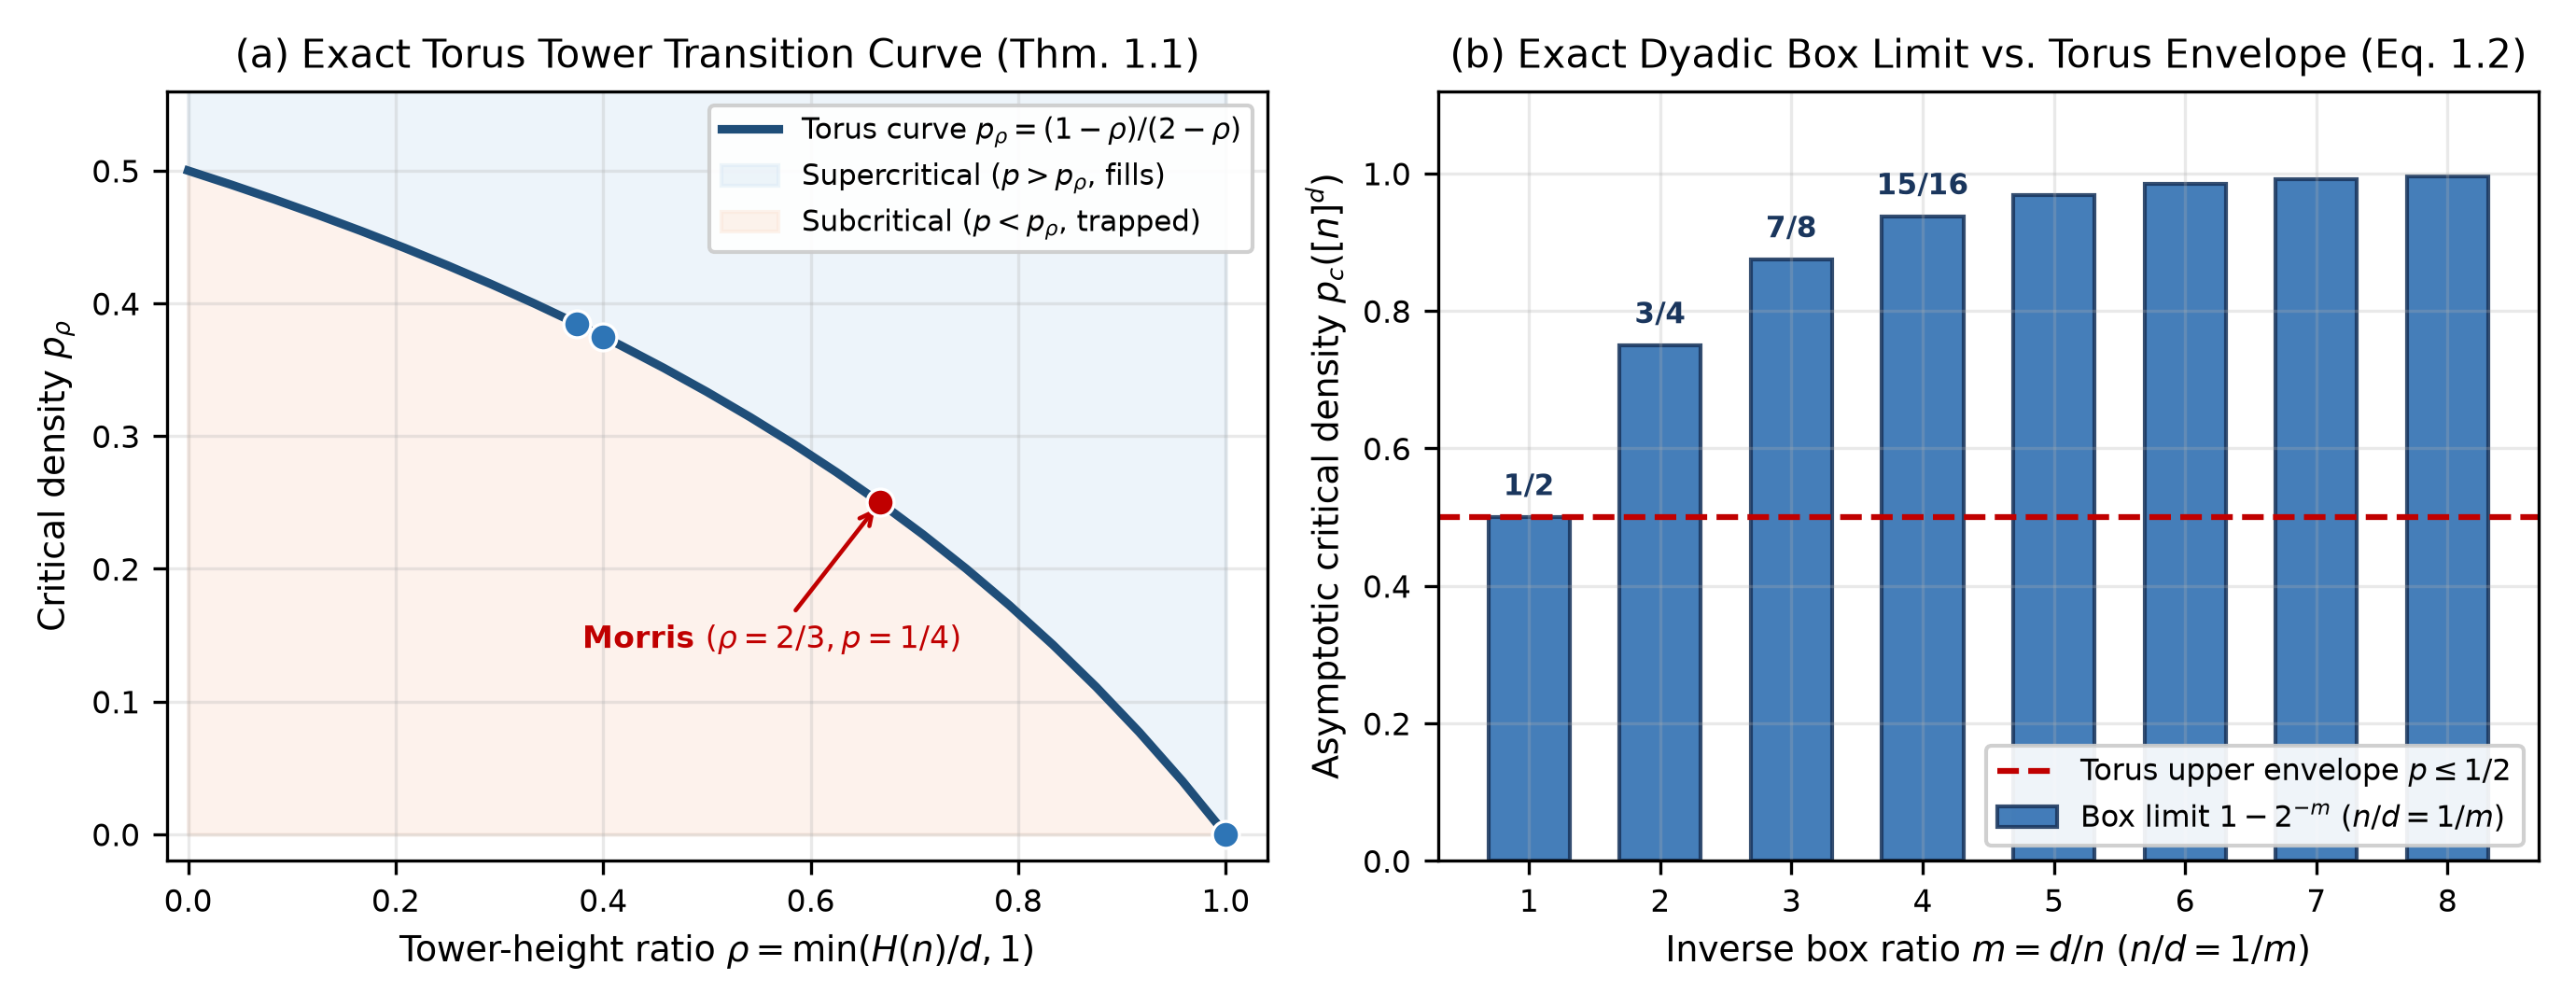
\includegraphics[width=\columnwidth]{../figures/fig1_tower_curve_and_box_gap.png}
  \caption{(a) Exact-$\QQ$ Theorem~1.1 torus tower curve $p_\rho = (1-\rho)/(2-\rho)$ with Morris's $(2/3,1/4)$ point and certified Mode~1 instances. (b) Sharp Eq.~(1.2) dyadic box limit $1-2^{-m}$ strictly exceeding the torus envelope $p \le 1/2$ for all $m \ge 2$.}
  \label{fig:tower}
\end{figure}

\paragraph{Tower Curve and Dyadic Box Gap (Fig.~\ref{fig:tower}).}
Mode~1 replays Morris's exact benchmark at $d=6, n=65536$ ($H(65536)=4, \rho=2/3, p_\rho=1/4$, $0.051\,\mathrm{ms}$), intermediate points $(d=8, n=16) \mapsto (3/8, 5/13)$ and $(d=10, n=65536) \mapsto (2/5, 3/8)$, and the saturated boundary $(d=4, n=65536) \mapsto (1, 0)$ ($0.036\,\mathrm{ms}$). Mode~4 pairs the exact dyadic box limits $1/2, 3/4, 7/8, 15/16$ ($m=1..4$) with Lemma~2.3 separated-rectangle configurations in $d=2,3,4$ attaining exact pairwise separations $\ell_\infty \in \{3, 6, 6, 8\} > 2t$ ($0.061$--$0.072\,\mathrm{ms}$).

\begin{figure}[t]
  \centering
  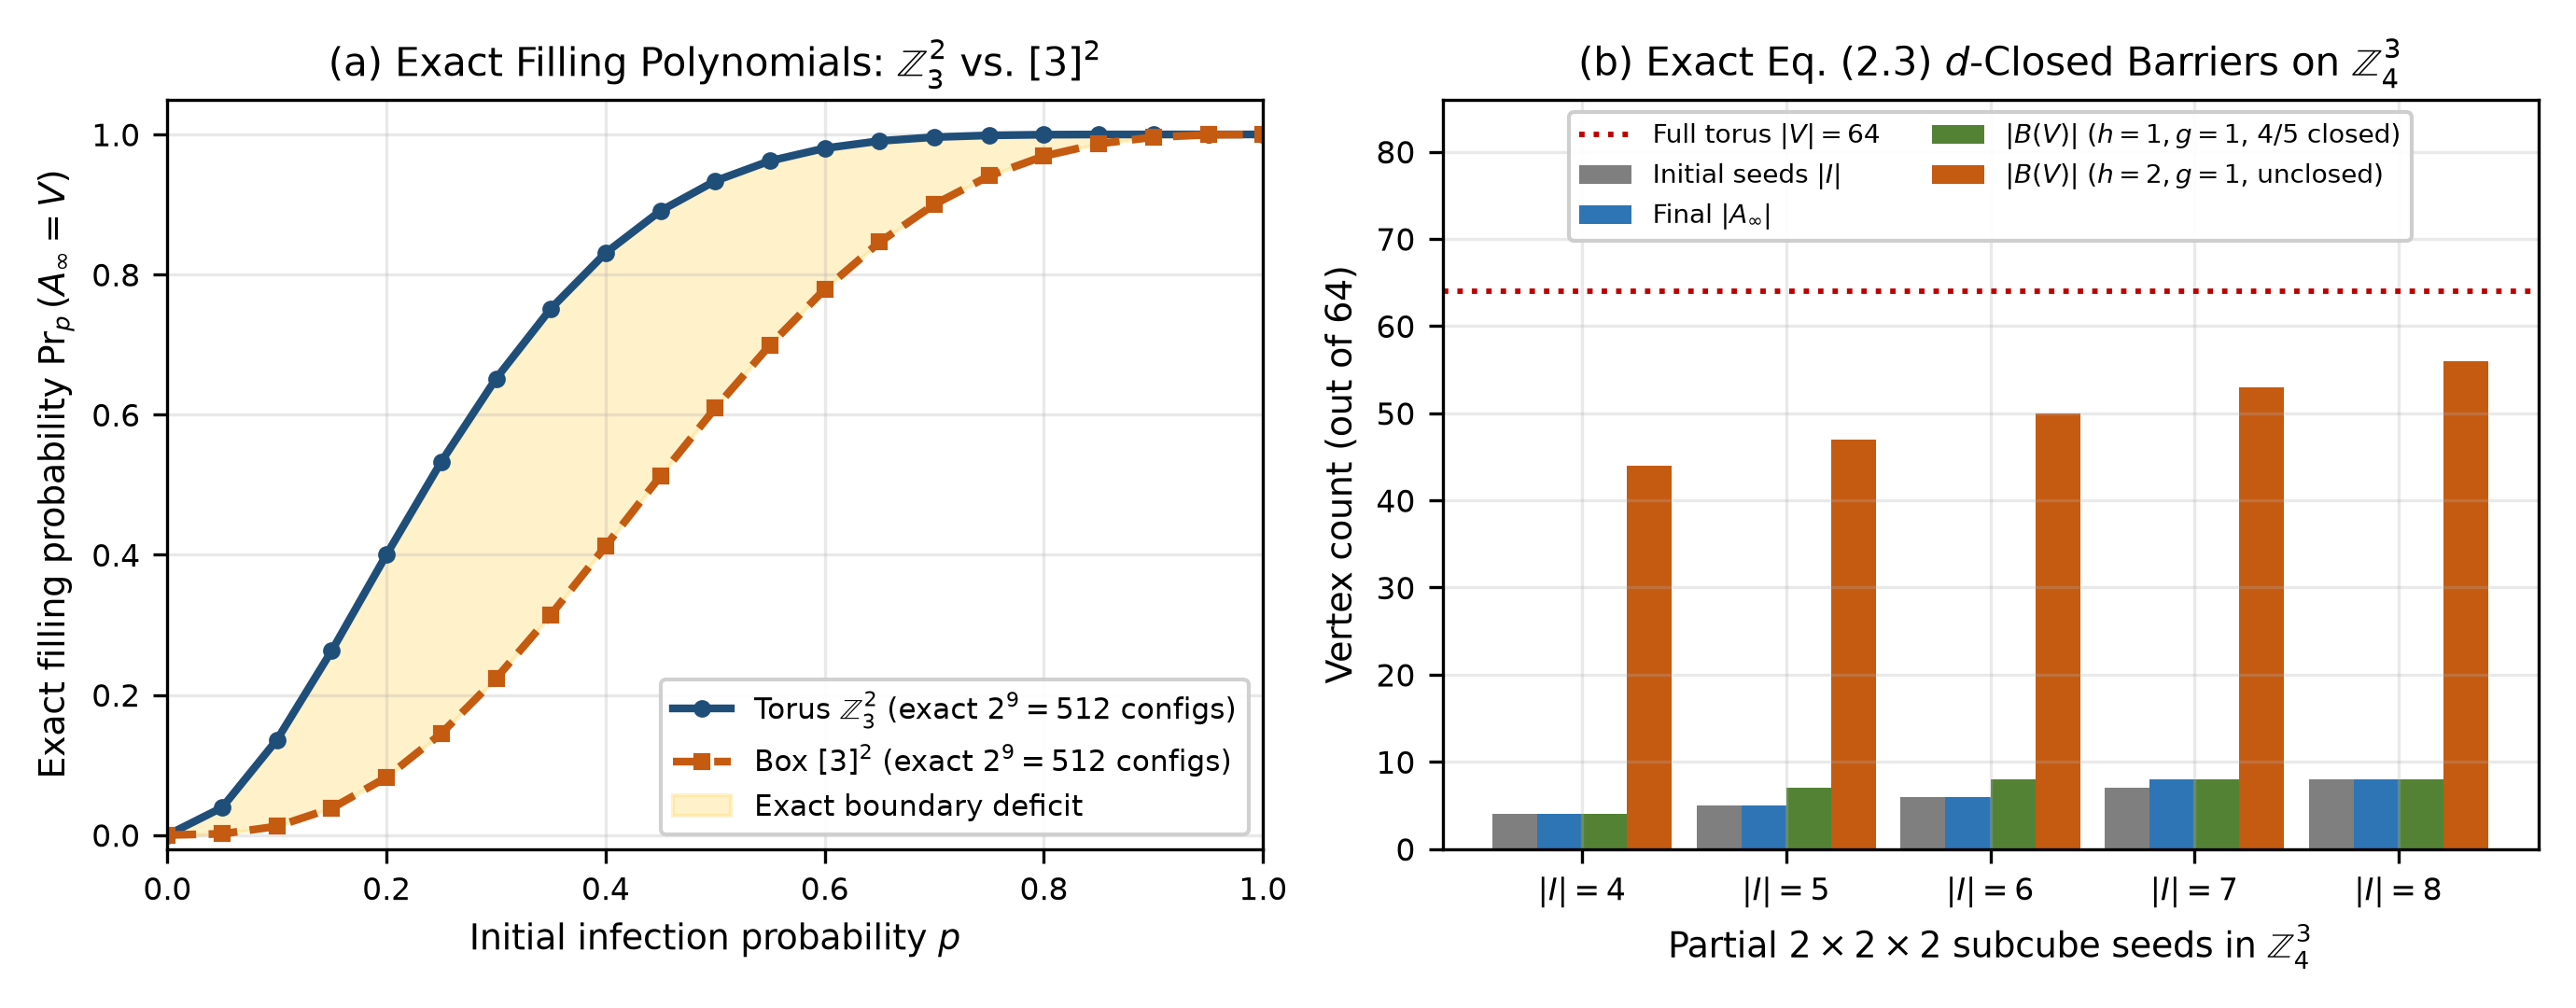
\includegraphics[width=\columnwidth]{../figures/fig2_exact_filling_and_eq23_barriers.png}
  \caption{(a) Exact filling probability polynomials over all $2^9 = 512$ configurations on $\ZZ_3^2$ vs.\ $[3]^2$, quantifying the finite boundary deficit. (b) Exact Eq.~(2.3) barrier census on $\ZZ_4^3$ ($|V|=64$) for $2\times 2\times 2$ subcube prefixes of sizes $4..8$.}
  \label{fig:filling}
\end{figure}

\paragraph{Exact Filling Polynomials and Eq.~(2.3) Barriers (Fig.~\ref{fig:filling}).}
Exhaustive enumeration over all $2^9=512$ initial configurations on $\ZZ_3^2$ vs.\ $[3]^2$ yields exact rational filling polynomials: at $p=1/4$, $\Pr_{1/4}(\text{fills}) = 17459/32768 \approx 0.5328$ on $\ZZ_3^2$ versus $18995/131072 \approx 0.1449$ on $[3]^2$; at $p=1/2$, $239/256 \approx 0.9336$ versus $39/64 = 0.6094$, directly reflecting the corner degree deficit $d$ vs.\ $2d$. In Mode~2, $\ZZ_6^2$ fills from a 6-site diagonal in 3 rounds ($0.108\,\mathrm{ms}$) and $\ZZ_4^3$ fills in 2 rounds ($0.175\,\mathrm{ms}$), while punctured subcubes on $\ZZ_4^3$ ($7 \to 8$ sites) and $[3]^4$ ($14 \to 16$ sites) are certified trapped by tight Eq.~(2.3) $d$-closed barriers ($|A_\infty|=|B(V)| < |V|$, $0.365$--$0.446\,\mathrm{ms}$). Our $\ZZ_4^3$ subcube-prefix census (Fig.~\ref{fig:filling}b) reveals a sharp budget trade-off: $h=1, g=1$ ($d-hg=2$) certifies tight closure ($|B|=4$ or $8$) on $4/5$ prefixes (failing only on the asymmetric 5-seed prefix), whereas $h=2, g=1$ ($d-hg=1$) over-expands to $44$--$56$ vertices without closing.

\begin{figure}[t]
  \centering
  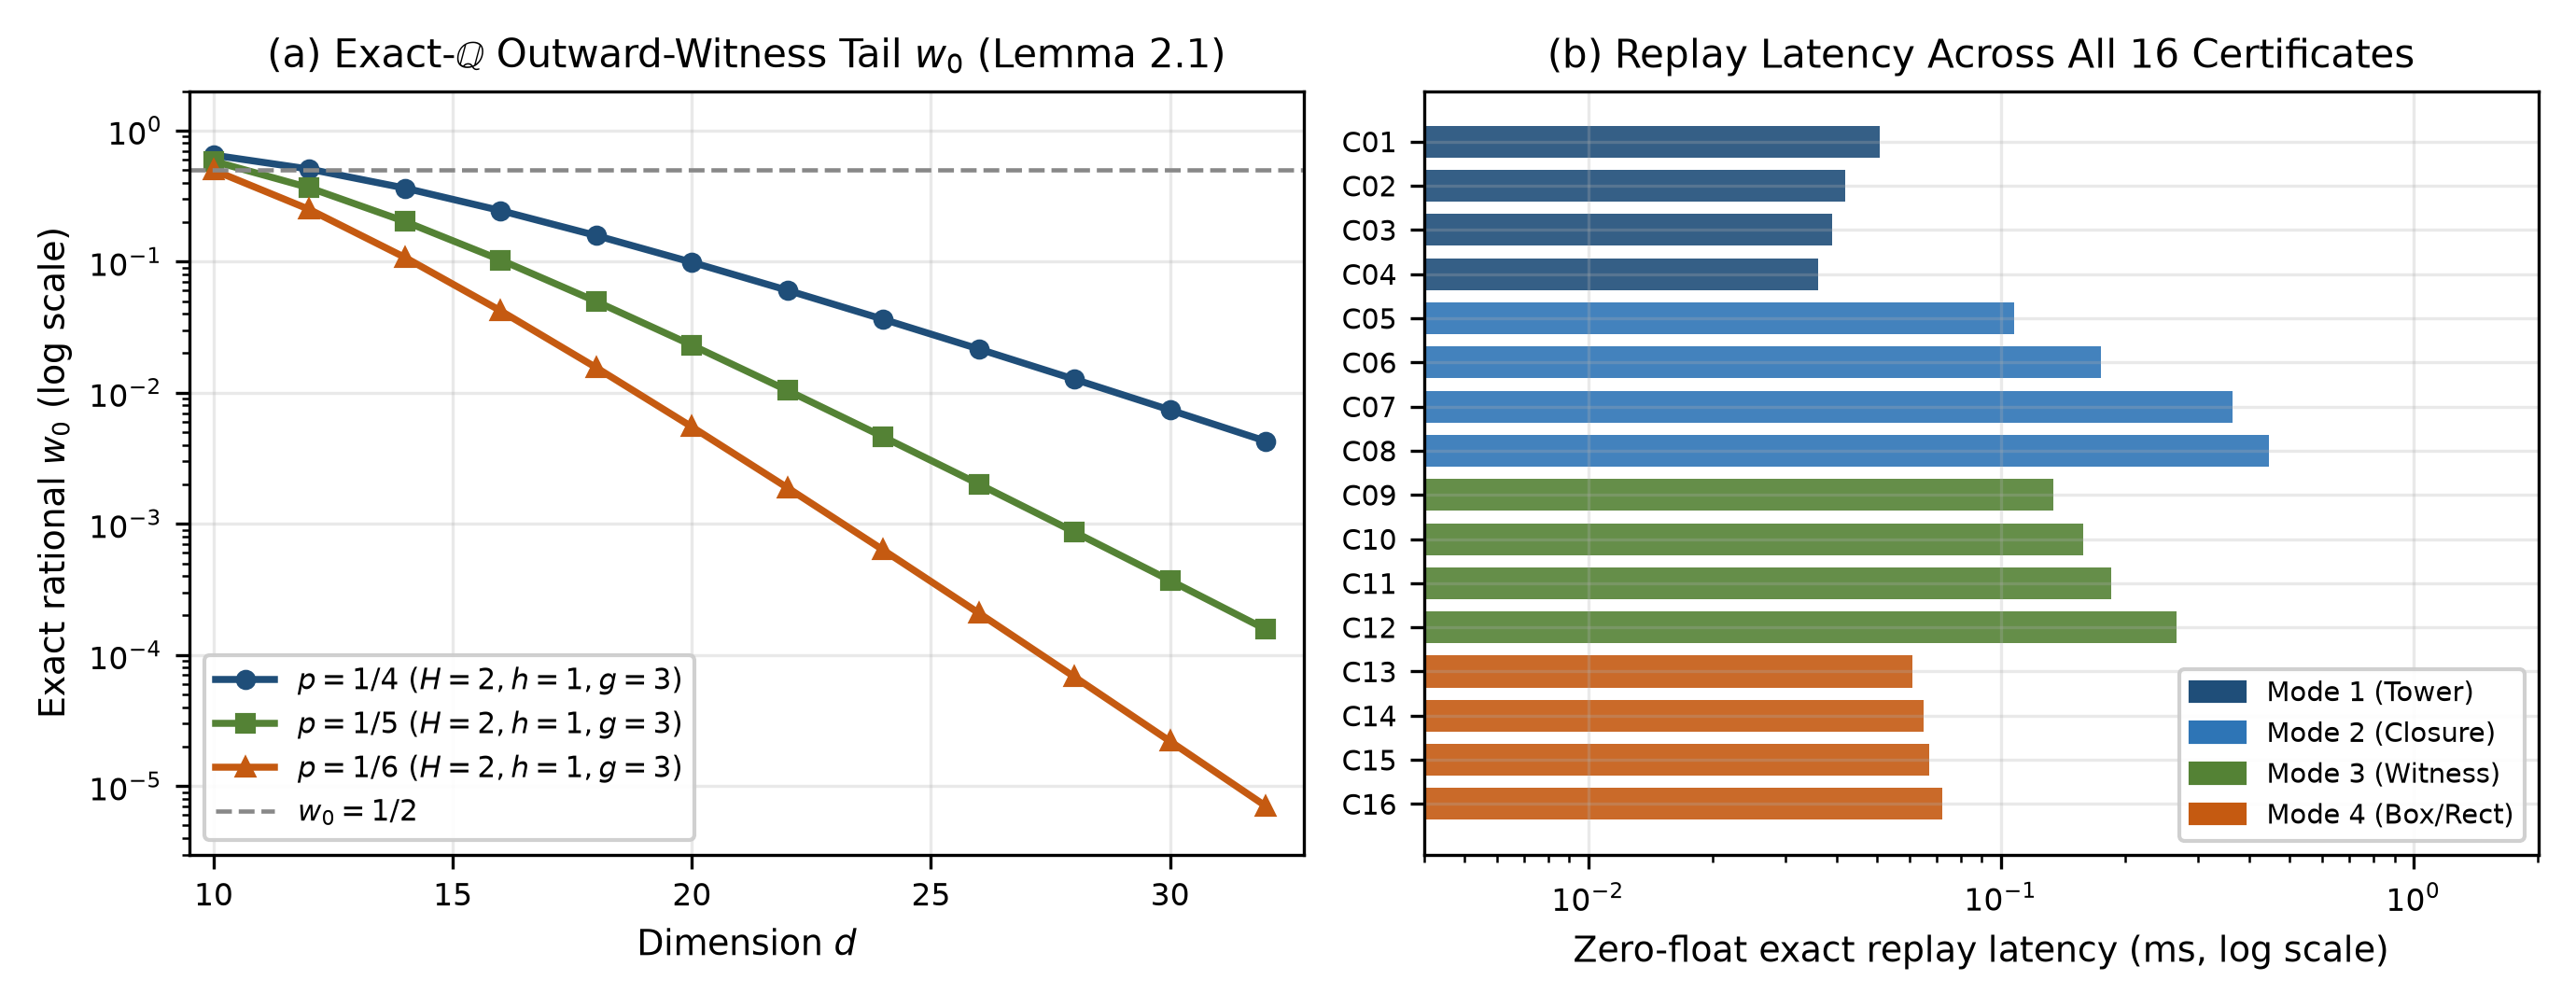
\includegraphics[width=\columnwidth]{../figures/fig3_outward_witness_and_replay_latency.png}
  \caption{(a) Exact-$\QQ$ Lemma~2.1 outward-witness probability $w_0(d,p)$ across $d=10..32$ ($H=2,h=1,g=3$). (b) Zero-float replay latency across all 16 canonical \texttt{BOOTSTRAP-TOWER-CERT-1.0} certificates ($0.036$--$0.446\,\mathrm{ms}$).}
  \label{fig:w0}
\end{figure}

\paragraph{Exact-$\QQ$ Outward-Witness Decay and Red-Team Audit (Fig.~\ref{fig:w0}, Table~\ref{tab:replay}).}
In Mode~3, exact rational evaluation of Eq.~\eqref{eq:w0} certifies $w_0 < 1/2$ across $d \in \{16, 20, 24, 30\}$ with exact numerators up to $141$~bits in $0.134$--$0.266\,\mathrm{ms}$. Across $d=10..32$ ($H=2,h=1,g=3$), $w_0$ decays exponentially from $0.4978$ ($d=10$) to $7.036\times 10^{-6}$ ($d=32$, exact 145-bit numerator) at $p=1/6$. Finally, our adversarial test suite (\texttt{tests/test\_suite.py}) mounts 60 live forgery attacks—including float injection, bool-as-int type confusion, unreduced fractions, huge-denominator DoS, false filling claims, unclosed Eq.~(2.3) barriers, violated $g > 2h$ margins, duplicate/uncovered marks, and $\ell_\infty \le 2t$ rectangle collisions—achieving \textbf{60/60 rejections} with zero bypasses.

\begin{table}[t]
\centering
\caption{Summary of all 16 canonical \texttt{BOOTSTRAP-TOWER-CERT-1.0} certificates and 60/60 live adversarial red-team audit.}
\label{tab:replay}
\resizebox{\columnwidth}{!}{%
\begin{tabular}{@{}lccc@{}}
\toprule
Verification Mode & Certs & Latency (ms) & Attacks Rejected \\
\midrule
Mode~1: Tower-Curve Bijection & 4 & $0.036$--$0.051$ & 10/10 \\
Mode~2: Dynamics \& Eq.~(2.3) Barrier & 4 & $0.108$--$0.446$ & 16/16 \\
Mode~3: Outward-Witness Tail $w_0$ & 4 & $0.134$--$0.266$ & 10/10 \\
Mode~4: Dyadic Box \& Rectangles & 4 & $0.061$--$0.072$ & 12/12 \\
Global Schema / Type / Rational & -- & -- & 12/12 \\
\midrule
\textbf{Total} & \textbf{16} & \textbf{0.036--0.446} & \textbf{60/60} \\
\bottomrule
\end{tabular}}
\end{table}

\section{Conclusion}
We have delivered a zero-dependency 18-theorem Lean~4 kernel and an exact-$\QQ$ certificate auditor for the finite algebraic, barrier-closure, outward-witness, and geometric core of Koval and Peres's tower transition in majority bootstrap percolation~\cite{koval2026tower}. Extending the Lean~4 formalization to quantitative Azuma--Hoeffding / Talagrand concentration bounds and multi-scale renormalization couplings remains an attractive direction for future formalized probability.

\bibliographystyle{plain}
\bibliography{references}
\end{document}
